\section{Kvocientni prostori}
\subsection{Kvocientna topologija}
\begin{definicija}
    Naj bo \(X\) množica, \(\sim\) ekvivalenčna relacija na \(X\). 
    \begin{itemize}
        \item Za poljuben \(x \in X\) označimo \([x] = \setb{y \in X}{y \sim x}\) \df{ekvivalenčni razred}, ki pripada \(x\).
        \item \df{Kvocientna množica} množice \(X\) po relacije \(\sim\) je množica vseh ekvivalenčnih razredov \(\setb{[x]}{x \in X} =: X/_\sim\).
        \item Preslikava \(q: X \to X/_\sim, \ q(x) = [x]\) je \df{kvocientna projekcija}.
    \end{itemize}    
\end{definicija}

\begin{opomba}
    Ekvivalenčni razredi predstavljamo kot točke.
\end{opomba}

\begin{primer}
    Naj bo \(X = [0, 1]\). Ekvivalenčna relacija \(\sim\) določna z \[0 \sim 1 \quad (1 \sim 0, \all{x \in X}x \sim x).\]
    Kako si lahko predstavljamo kvocientno množico \(X/_\sim\)? Bodisi kot interval \([0,1)\) bodisi kot krožnico.
    \begin{center}
        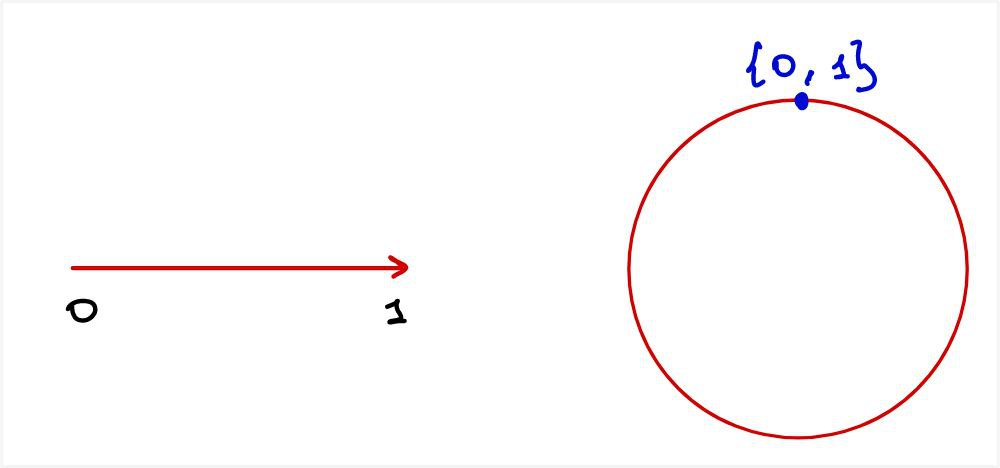
\includegraphics[width=0.5\textwidth]{img/01_001.jpg}      
    \end{center}
\end{primer}

\begin{opomba}
    \
    \begin{itemize}
        \item Pri opisu ekvivalenčne relacije bomo običajno navedli le netrivialne relacije, ki generirajo ekvivalenčno relacijo, ob upoštevanju lastnosti ekvivalenčnih relacij.
        \item Ekvivalenčna relacija \(\sim\) na \(X\) določna razdelitev množice \(X\) na ekvivalenčne razrede. To razdelitev označimo z \(\mathcal{R} = \setb{[x]}{x \in X} \subseteq P(X)\). Kvocientno množico lahko označimo z \(X/_\sim = X/_\mathcal{R}\).
        \item Če \(\sim\) določna le en netrivialen ekvivalenčni razred \(A \subseteq X, \ |A| \neq 1\), potem kvocientno množico označimo z \(X/_A\).
    \end{itemize}
\end{opomba}

Če je \(X\) topološki prostor in \(\sim\) ekvivalenčna relacija na \(X\), želimo \(X/_\sim\) opremiti z topologijo tako, da bo ta odražala lastnosti prostora \(X\). Posebej želimo, da je kvocientna projekcija \(q: X \to X/_\sim\) zvezna.

Pogoj \[\all{\op{V} \subseteq \qs{X}} \op{\invimg{q}(V)} \subseteq X\] topologije na \(\qs{X}\) ne določna enolično -- če neka topologija na \(\qs{X}\) temu ustreza, ustreza tudi vsaka šibkejša. Zato je \(\qs{X}\) smiselno opremiti z najmočnejšo topologijo, pri kateri je \(q\) zvezna. Torej za odprte množice v \(\qs{X}\) vzamemo vse, ki imajo odprte praslike v \(X\).

\begin{definicija}
    Naj bo \((X, \T)\) topološki prostor in \(\sim\) ekvivalenčna relacija na \(X\).
    \begin{itemize}
        \item \df{Kvocientna topologija} na \(\qs{X}\) je \[\T_\sim = \setb{V \subseteq \qs{X}}{\invimg{q}(V) \subseteq X \ \text{odprta}}.\]
    \end{itemize}
\end{definicija}

\begin{trditev}
    \(\T_\sim\) je topologija na \(\qs{X}\).
\end{trditev}

\begin{opomba}
    V kvocientni topologiji na \(\qs{X}\) velja:
    \[\op{V} \subseteq \qs{X} \liff \op{\invimg{q}(V)} \subseteq X.\]
    \((\Rightarrow)\) je zveznost preslikave \(q\);

    \((\Leftarrow)\) je največjost \(\T_\sim\).

    Velja tudi: 
    \[\cl{Z} \subseteq \qs{X} \liff \cl{\invimg{q}(Z)} \subseteq X.\]
\end{opomba}

\begin{primer}
    Ali je torej \(q\) odprta in zaprta? Ni nujno!
    \begin{itemize}
        \item Naj bo \(X = [0,1], \ \mathcal{R} = \set{[0, 1), {1}}\). Kaj je \(\q{X}{\mathcal{R}}\)? Ali sta \(\set{[0]}\) in \(\set{[1]}\) odprti? Ali je \(q\) zaprta?
        \item Naj bo \(X = [0,2], \ [1, 2] \ \text{edini netrivialni ekvivalenčni razred}\). Kaj je \(\q{X}{[1, 2]}\)? Ali je \(q\) odprta?
        \item Naj bo \(X = [0, 1], \ A = X \cap \Q, \ B = X \setminus \Q\). Kaj je \(\q{X}{\set{A, B}}\)? Kaj je kvocientna topologija?
    \end{itemize}
\end{primer}

\newpage
\begin{definicija}
    Naj bo \(X\) množica in \(\sim\) ekvivalenčna relacija. 
    \begin{itemize}
        \item Za \(A \subseteq X\) je njeno \df{nasičenje} enako \[\invimg{q}(\img{q}(A)) = \bigcup \setb{B \in \qs{X}}{A \cap B \neq \emptyset}.\]
    \end{itemize}
\end{definicija}

\begin{trditev}
    Naj bo \(X\) topološki prostor, \(\sim\) ekvivalenčna relacija, \(A \subseteq X\). Velja:
    \begin{itemize}
        \item \(\img{q}(A) \ \text{je odprta/zaprta} \liff  \text{nasičenje} \ \invimg{q}(\img{q}(A)) \ \text{odprto/zaprto}\). 
        \item \(\all{\op{U} \subseteq X} \invimg{q}(\img{q}(U)) \ \text{odprto/zaprto} \lthen q \ \text{je odprta/zaprta}\).
    \end{itemize}
\end{trditev}

\paragraph{Cilj} Imamo nek topološki prostor \(X\) in ekvivalenčno relacijo \(\sim\). Če je to mogoče, želimo poiskati nek geometrični model \(Y\) za kvocient \(\qs{X}\) in jasno pokazati, da je \(\qs{X} \approx Y\).

\begin{primer}
    \
    \begin{itemize}
        \item Naj bo \(X = \R, \ A = \Z\). Kaj je \(\q{\R}{A}\)?
        \item Naj bo \(X = [0,1], \ A = \setb{\frac{1}{n}}{n \in \N} \cup \set{0}\). Kaj je \(\q{\R}{A}\)? Ali je kompakten?
    \end{itemize}
    V obeh primerih imamo števno mnogo krožnic, spetih v eni točki. Ali sta ta prostora homeomorfna?
\end{primer}

\subsection{Kvocientne preslikave}
\paragraph{Cilj} Razumeti preslikave iz kvocientov.

Naj bo \(X\) topološki prostor, \(\sim\) ekvivalenčna relacija.

\[
    \begin{tikzcd}
        X \arrow[swap]{d}{q} \arrow{rd}{f \, := g \,  \circ \, q} &   \\%
        X/_\sim \arrow[swap]{r}{g} & Y
    \end{tikzcd}
\]

Zvezna preslikava \(g: \qs{X} \to Y\) določa zvezno preslikavo \(f = g \circ q: X \to Y\).

Če je \(x \sim y\) v \(X\), je \([x] = q(x) = q(y) = [y]\) in zato je \(f(x) = g(q(x)) = g(q(y)) = f(y)\). Torej ta \(f\) je konstantna na ekvivalenčnih razredih, tj. ekvivalentne točke slika v iste.

Želimo obratno: za preslikavo \(f: X \to Y\) poiskati pogoje, da določa preslikavo iz \(\qs{X}\) v \(Y\).
%
\[
    \begin{tikzcd}
        X \arrow{r}{f} \arrow[swap]{d}{q} & Y \\
        \qs{X} \arrow[dashed, swap]{ru}{\overline{f}}
    \end{tikzcd}
\]
%
Če naj diagram komutira, mora biti \(f\) konstantna na ekvivalenčnih razredih:
\[
    \all{x,y \in X} x \sim y \lthen f(x) = f(y).
\]

Če to velja, potem definiramo \[\overline{f}([x]) := f(x).\]
\(\overline{f}\) je preslikava, inducirana s \(f\).

\begin{trditev}
    Naj bo \(X\) topološki prostor, \(\sim\) ekvivalenčna relacija, \(f: X \to Y\) zvezna preslikava, ki je konstantna na ekvivalenčnih razredih. Potem \(f\) določa dobro definirano preslikavo \[\overline{f}: \qs{X} \to Y,\] za katero velja: \[\overline{f} \circ q = f.\]
    Poleg tega velja:
    \begin{itemize}
        \item Če je \(f\) zvezna, potem je tudi \(\overline{f}\) zvezna.
        \item Če je \(f\) surjektivna, je \(\overline{f}\) surjektivna.
        \item Če za \(\all{x, y \in X} x \not \sim y \lthen f(x) \neq f(y)\), potem je \(\overline{f}\) injektivna, tj. \(f\) loči ekvivalenčne razrede.
    \end{itemize}
\end{trditev}

\begin{proof}
    Definicija kvocientne topologije.
\end{proof}

\newpage
Zanima nas, kdaj bo \(\overline{f}\) homeomorfizem. Velja:

\(\overline{f}: \qs{X} \to Y\) je homeomorfizem, če 
\begin{itemize}
    \item zvezna, bijektivna in inverz zvezen oz.
    \item bijekcija iz \(\qs{X}\) v \(Y\) in porodi bijekcijo med topologiji na \(\qs{X}\) in \(Y\).
\end{itemize}
Torej NTSE
\begin{itemize}
    \item \(\overline{f}\) je homeomorfizem.
    \item \(\overline{f}\) je bijekcija iz \(\qs{X}\) v \(Y\) in porodi bijekcijo med odprtimi množici.
    \item \(\overline{f}\) je bijekcija in velja: \[\all{V \subseteq Y} V \ \text{je odprta} \liff \op{\invimg{\overline{f}}(V)} \subseteq \qs{X} \liff \op{\invimg{f}(V)} =  \op{\invimg{q}(\invimg{\overline{f}}(V))} \subseteq X.\]
\end{itemize}

\begin{definicija}
    Naj bosta \(X, Y\) topološka prostora in \(f: X \to Y\) preslikava. Če je \(f\) surjektivna in če 
    \[\all{V \subseteq Y} V \ \text{je odprta} \liff \invimg{f}(V) \subseteq X \ \text{je odprta},\]
    potem \(f\) imenujemo \df{kvocientna preslikava}.
\end{definicija}

\begin{opomba}
    \
    \begin{itemize}
        \item Po definiciji kvocientne topologiji, je kvocientna projekcija kvocientna preslikava. 
        
        Obratno: vsako kvocientno preslikavo \(f: X \to Y\) lahko obravnavamo kot kvocientno projekcijo pri ekvivalenčni relaciji, določeni z razbitjem \(X\) na praslike točk.
        \item Kvocientna preslikava je vedno zvezna, ni pa nujno odprta niti zaprta.
        \item Implikacija \((\Leftarrow)\) v definiciji kvocientne preslikave je posebna lastnost, tej včasih rečemo \df{kvocient v ožjem smislu}.
        
        Za zvezno surjekcijo je za njeno kvocientnost potrebno preveriti le ta pogoj.
        \item Surjektivna preslikava \(f\) je kvicientna natanko tedaj, ko 
        \[\all{Z \subseteq Y} Z \ \text{je zaprta} \liff \invimg{f}(Z) \subseteq X \ \text{je zaprta},\]
    \end{itemize}
\end{opomba}

\begin{lema}
    Naj bo \(f: X \to Y\) zvezna in surjektivna. Če je \(f\) odprta ali zaprta, je kvocientna.
\end{lema}

\begin{proof}
    Preveriti je treba le kvocientnost v ožjem smislu.
\end{proof}

\begin{izrek}[O prepoznavi kvocienta]
    Naj bosta \(X, Y\) topološka prostora in \(\sim\) ekvivalenčna relacija na \(X\). Naj bo \(f:~X~\to~Y\) kvocientna preslikava, ki naredi enake identifikacije kot \(\sim\), tj.\ \(f\) je konstantna na ekvivalenčnih razredih in loči ekvivalenčne razrede:
    \[\all{x, y \in X} x \sim y \liff f(x) = f(y).\]
    Potem je inducirana preslikava \(\overline{f}: \qs{X} \to Y\) homeomorfizem.
\end{izrek}